

\section{Results and discussion}
\label{sec:discussion}

\begin{table}[!t]
\centering
\caption{Effect of graded similarity labels on batch composition and model training.}
\label{tab:msls-labels-effect}
\resizebox{\textwidth}{!}{%
\setlength\tabcolsep{1.5pt}

\begin{tabular}{@{}l@{\hspace{4\tabcolsep}}l@{\hspace{4\tabcolsep}}c@{\hspace{8\tabcolsep}}ccc@{\hspace{8\tabcolsep}}ccc}
 &  &  & \multicolumn{3}{c}{\textbf{MSLS-Val}} & \multicolumn{3}{c}{\textbf{MSLS-Test}} \\

\textbf{Method} & \textbf{Loss} & \textbf{Batch}  & \textbf{R@1} &\textbf{ R@5} & \textbf{R@10} & \textbf{R@1} & \textbf{R@5} & \textbf{R@10}  \\
\toprule
VGG-GeM & CL & binary  &  47.0 & 60.3 & 65.5 & 27.9 & 40.5 & 46.5  \\
VGG-GeM & GCL & binary  &  57.4 & 73.4 & 76.9 & 35.9 & 49.3 & 57.8  \\ \midrule
VGG-GeM & CL & graded  &  45.8 & 60.1 & 65.1 & 28.0 & 40.8 & 47.0  \\
VGG-GeM & GCL & graded  &  65.9 & 77.8 & 81.4 & 41.7 & 55.7 & 60.6  \\
 \bottomrule
\end{tabular}
}
\end{table}

\noindent\textbf{Graded similarity for batch composition and model training.} We carry out a baseline experiment to evaluate the impact of the new graded similarity labels on the effectiveness of the learned descriptors. We analyze their contribution to the composition of the batches, and directly to the training of the network by using them in combination with the proposed GCL. We first consider the traditional binary labels only, and compose batches by balancing positive and negative pairs. Subsequently, we compose the batches by considering the new graded similarity labels, and select $50\%$ of positive pairs (similarity higher than $50\%$), $25\%$ of soft negative samples (similarity higher than $0\%$ and lower than $50\%$) and $25\%$ of hard negatives ($0\%$ similarity). 

In Table~\ref{tab:msls-labels-effect}, we report the results using a VGG16 backbone on the MSLS dataset. These results demonstrate that the proposed graded similarity labels are especially useful for training descriptors that perform better in nearest neighbor search retrieval, and also contribute to form better balanced batches to exploit the data in a more efficient way. In the following, all experiments use the batch composition based on graded similarity.





\begin{table*}[t!]
\centering
\renewcommand{\arraystretch}{1}
\caption{Comparison to state-of-the-art methods on benchmark datasets. All methods are trained on the MSLS training set. Our top results are underlined, while overall best results are in bold. Methods using re-ranking are in the middle part of the table and marked with $^\star$.}
\label{tab:msls-sota}

\resizebox{\textwidth}{!}{%
\setlength\tabcolsep{1.5pt}
\revised{
\begin{tabular}{@{}lcc@{\hspace{4\tabcolsep}}ccc@{\hspace{4\tabcolsep}}ccc@{\hspace{4\tabcolsep}}ccc@{\hspace{4\tabcolsep}}ccc@{\hspace{4\tabcolsep}}ccc@{\hspace{4\tabcolsep}}ccc@{}}
 &  &  & \multicolumn{3}{c}{\textbf{MSLS-Val}} & \multicolumn{3}{c}{\textbf{MSLS-Test}} & \multicolumn{3}{c}{\textbf{Pitts30k}} & \multicolumn{3}{c}{\textbf{Tokyo24/7}} & \multicolumn{3}{c}{\textbf{RobotCar Seasons v2}} & \multicolumn{3}{c}{\textbf{Extended CMU Seasons}} \\ 
\textbf{Method} & \textbf{PCA$_w$} & \textbf{Dim} & \textbf{R@1} & \textbf{R@5} & \textbf{R@10} & \textbf{R@1} & \textbf{R@5} & \textbf{R@10} & \textbf{R@1} & \textbf{R@5} & \textbf{R@10} & \textbf{R@1} & \textbf{R@5 }& \textbf{R@10} & \textbf{.25m/2$\degree$} & \textbf{.5m/5$\degree$ }& \textbf{5m/10$\degree$ }& \textbf{.25m/2$\degree$ }& \textbf{.5m/5$\degree$ }& \textbf{5m/10$\degree$} \\\toprule 
%NetVLAD 64 Pitts & N & 32768 & 47.7 & 62.8 & 70.9 & 30.7 & 41.9 & 46.4 & 82.1 & 91.4 & 93.8 & 62.2 & 73.7 & 78.4 & 5.6 & 22.0 & 71.0 & 10.7 & 27.8 & 84.1 \\
%NetVLAD 64 Pitts & Y & 4096 & 70.7 & 81.4 & 84.6 & 30.6 & 41.9 & 47.5 & 83.7 & 91.8 & 94.0 & 67.0 & 77.8 & 80.3 & 5.8 & 23.1 & 73.2 & 11.6 & 30.3 & 87.5 \\
NetVLAD 64  & N & 32768 & 44.6 & 61.1 & 66.4 & 28.8 & 44.0 & 50.7 & 40.4 & 64.5 & 74.2 & 11.4 & 24.1 & 31.4 & 2.0 & 9.2 & 45.5 & 1.3 & 4.5 & 31.9 \\
NetVLAD 64  & Y & 4096 & 70.1 & 80.8 & 84.9 & 45.1 & 58.8 & 63.7 & 68.6 & 84.7 & 88.9 & 34.0 & 47.6 & 57.1 & 4.2 & 18.0 & 68.1 & 3.9 & 12.1 & 58.4 \\
NetVLAD 16  & N & 8192 & 49.5 & 65.0 & 71.8 & 29.3 & 43.5 & 50.4 & 48.7 & 70.6 & 78.9 & 13.0 & 33.0 & 43.8 & 1.8 & 9.2 & 48.4 & 1.7 & 5.5 & 39.1 \\
NetVLAD 16  & Y & 4096 & 70.5 & 81.1 & 84.3 & 39.4 & 53.0 & 57.5 & 70.3 & 84.1 & 89.1 & 37.8 & 53.3 & 61.0 & 4.8 & 17.9 & 65.3 & 4.4 & 13.7 & 61.4 \\
 
TransVPR~\cite{wang2022transvpr} & - & - & 70.8 & 85.1 & 86.9 & 48 & 67.1 & 73.6 & 73.8 & 88.1 & 91.9 & - & - & - & 2.9 & 11.4 & 58.6 & - & - & - \\ \hline
 
SP-SuperGlue$^\star$~\cite{sarlin20superglue} & - & - & 78.1 & 81.9 & 84.3 & 50.6 & 56.9 & 58.3 & 87.2 & 94.8 & 96.4 & 88.2 & 90.2 & 90.2 & 9.5 & \bfseries 35.4 & 85.4 & 9.5 & 30.7 & \textbf{96.7} \\
DELG$^\star$~\cite{delg} & - & - & 83.2 & 90.0 & 91.1 & 52.2 & 61.9 & 65.4 & \bfseries 89.9 & \bfseries 95.4 & \bfseries 96.7 & \bfseries 95.9 & \bfseries 96.8 & \bfseries 97.1 & 2.2 & 8.4 & 76.8 & 5.7 & 21.1 & 93.6 \\

Patch NetVLAD$^\star$~\cite{hausler2021patch} & Y & 4096 & 79.5 & 86.2 & 87.7 & 48.1 & 57.6 & 60.5 & 88.7 & 94.5 & 95.9 & 86.0 & 88.6 & 90.5 & 9.6 & 35.3 & \textbf{90.9} & \textbf{11.8} & \textbf{36.2} & 96.2 \\

TransVPR$^\star$~\cite{wang2022transvpr} & - & - & \textbf{86.8} & \textbf{91.2} & 92.4 & \textbf{63.9} & 74 & 77.5 & 89 & 94.9 & 96.2 & - & - & - & \textbf{9.8} & 34.7 & 80 & - & - & - \\ \midrule
%ResNet101-AP-GeM & Y & 2048 & 64.1 & 75.0 & 78.2 & 33.7 & 44.5 & 49.4 & 80.7 & 91.4 & 94.0 & 11.4 & 22.9 & 30.5 & 5.1 & 20.5 & 66.1 & 4.9 & 14.7 & 65.2 \\
%NetVLAD-SARE & Y & 4096 & 68.1 & 77.3 & 82.4 & 34.4 & 44.3 & 48.8 & 87.8 & 94.3 & \textbf{95.9} & 79.7 & 86.7 & 90.5 & 7.4 & 26.5 & 81.3 & 6.4 & 19.4 & 75.5 \\ \midrule
NetVLAD-GCL
 &
  N &
  32768 &
  62.7 &
  75.0 &
  79.1 &
  41.0 &
  55.3 &
  61.7 &
  52.5 &
  74.1 &
  81.7 &
  20.3 &
  45.4 &
  49.5 &
  3.3 &
  14.1 &
  58.2 &
  3.0 &
  9.7 &
  52.3 \\
NetVLAD-GCL
  &
  Y &
  4096 &
  63.2 &
  74.9 &
  78.1 &
  41.5 &
  56.2 &
  61.3 &
  53.5 &
  75.2 &
  82.9 &
  28.3 &
  41.9 &
  54.9 &
  3.4 &
  14.2 &
  58.8 &
  3.1 &
  9.7 &
  52.4 \\ 
VGG-GeM-GCL  & N & 512 & 65.9 & 77.8 & 81.4 & 41.7 & 55.7 & 60.6 & 61.6 & 80.0 & 86.0 & 34.0 & 51.1 & 61.3 & 3.7 & 15.8 & 59.7 & 3.6 & 11.2 & 55.8 \\
VGG-GeM-GCL  & Y & 512 & 72.0 & 83.1 & 85.8 & 47.0 & 60.8 & 65.5 & 73.3 & 85.9 & 89.9 & 47.6 & 61.0 & 69.2 & 5.4 & \underline{21.9} & 69.2 & 5.7 & 17.1 & 66.3 \\
ResNet50-GeM-GCL & N & 2048 & 66.2 & 78.9 & 81.9 & 43.3 & 59.1 & 65.0 & 72.3 & 87.2 & 91.3 & 44.1 & 61.0 & 66.7 & 2.9 & 14.0 & 58.8 & 3.8 & 11.8 & 61.6 \\
ResNet50-GeM-GCL & Y & 1024 & 74.6 & 84.7 & 88.1 & 52.9 & 65.7 & 71.9 & 79.9 & 90.0 & 92.8 & 58.7 & 71.1 & 76.8 & 4.7 & 20.2 & 70.0 & 5.4 & 16.5 & 69.9 \\
ResNet152-GeM-GCL& N & 2048 & 70.3 & 82.0 & 84.9 & 45.7 & 62.3 & 67.9 & 72.6 & 87.9 & 91.6 & 34.0 & 51.8 & 60.6 & 2.9 & 13.1 & 63.5 & 3.6 & 11.3 & 63.1 \\
ResNet152-GeM-GCL & Y & 2048 & 79.5 & 88.1 & 90.1 & 57.9 & 70.7 & 75.7 & \underline{80.7} & \underline{91.5} & \underline{93.9} & \underline{69.5} & \underline{81.0} & \underline{85.1} & \underline{6.0} & 21.6 & 72.5 & 5.3 & 16.1 & 66.4 \\
ResNeXt-GeM-GCL & N & 2048 & 75.5 & 86.1 & 88.5 & 56.0 & 70.8 & 75.1 & 64.0 & 81.2 & 86.6 & 37.8 & 53.6 & 62.9 & 2.7 & 13.4 & 65.2 & 3.5 & 10.5 & 58.8 \\
ResNeXt-GeM-GCL & Y & 1024 & \underline{ 80.9} & \underline{90.7} & \underline{\textbf{92.6}} & \underline{62.3} & \underline{\textbf{76.2}} & \underline{\textbf{81.1}} & 79.2 & 90.4 & 93.2 & 58.1 & 74.3 & 78.1 & 4.7 & 21.0 & \underline{74.7} & \underline{6.1} & \underline{18.2} & \underline{74.9} \\ \bottomrule

\end{tabular}
}}
\end{table*}







\noindent\textbf{Comparison with existing works.}
We compared our results with several place recognition works. We considered methods that use global descriptors like NetVLAD~\cite{Arandjelovic2017} (with 16 and 64 clusters in the VLAD layer) and methods based on two-stages retrieval and re-ranking pipelines, such as Patch-NetVLAD~\cite{hausler2021patch}, DELG~\cite{delg} and SuperGlue~\cite{sarlin20superglue}. We compared also against TransVPR~\cite{wang2022transvpr}, a transformer with and without a re-ranking stage. 
Table~\ref{tab:msls-sota} reports the results of our method in comparison to others. All the methods included in the table are based on backbones trained on the MSLS datasets. %, unless explicitly specified (i.e. the NetVLAD trained on Pittsburgh30k).  
The results of Patch-NetVLAD and TransVPR are taken from the respective papers, which also contain those of DELG and SuperGlue. 
%
When trained with VGG16 as backbone, our model (VGG16-GeM-GCL) obtains an absolute improvement of R@5
equal to 11.7\% compared to NetVLAD-64. 
This shows that the proposed graded similarity labels and the GCL function contribute to learn more powerful descriptors for place recognition, while keeping the complexity of the training process lower as hard-pair mining is not used. The result improvement holds also when the descriptors are post-processed with PCA whitening.

The data- and memory-efficiency of our pipeline allows us to easily train more powerful backbones, such as ResNeXt, that is instead tricky to do for other methods due to memory and compute requirements. Our ResNeXt+GCL outperforms the best method on the MSLS test set, namely TransVPR without re-ranking by 8.9\% and with re-ranking by 2.6\% (absolute improvement of R@5). It compares favorably with re-ranking based methods such as Patch-NetVLAD, DELG and SuperGLUE improving the R@5 by 18.6\%, 14.3\% and  18.3\%, respectively. 
We point out that we do not re-rank the retrieved images, and purposely keep the complexity of the steps at the strict necessary to perfom the VPR retrieval task. %which is a heavy post-processing procedure that relies on the retrieved images (during test).
We attribute our high results mainly to the effectiveness of the descriptors learned with the GCL function using the new graded similarity labels.





\begin{table*}[!t]
\centering
\caption{\revised{Ablation study on backbone, Contrastive (CL) vs Generalized Contrastive (GCL) loss, and PCA. All models are trained on MSLS.} }
\label{tab:msls-ablation}
\resizebox{\textwidth}{!}{%
\setlength\tabcolsep{1.5pt}
\revised{
\begin{tabular}{@{}llcc@{\hspace{4\tabcolsep}}ccc@{\hspace{4\tabcolsep}}ccc@{\hspace{4\tabcolsep}}ccc@{\hspace{4\tabcolsep}}ccc@{\hspace{4\tabcolsep}}ccc@{\hspace{4\tabcolsep}}ccc@{}}
 &  &  &  & \multicolumn{3}{c}{\textbf{MSLS-Val}} & \multicolumn{3}{c}{\textbf{MSLS-Test}} & \multicolumn{3}{c}{\textbf{Pitts30k}} & \multicolumn{3}{c}{\textbf{Tokyo24/7}} & \multicolumn{3}{c}{\textbf{RobotCar Seasons v2}} & \multicolumn{3}{c}{\textbf{Extended CMU Seasons}} \\

\textbf{Method} & \textbf{Loss} & \textbf{PCA$_w$} & \textbf{Dim} & \textbf{R@1} &\textbf{ R@5} & \textbf{R@10} & \textbf{R@1} & \textbf{R@5} & \textbf{R@10} &\textbf{ R@1} & \textbf{R@5} & \textbf{R@10} & \textbf{R@1} & \textbf{R@5 }& \textbf{R@10} & \textbf{0.25m/2$\degree$} & \textbf{0.5m/5$\degree$} & \textbf{5.0m/10$\degree$} & \textbf{0.25m/2$\degree$} & \textbf{0.5m/5$\degree$} & \textbf{5.0m/10$\degree$} \\
\toprule
\multirow{4}{*}{NetVLAD} &
  CL &
  N &
  32768 &
  38.5 &
  56.6 &
  64.1 &
  24.8 &
  39.1 &
  46.1 &
  24.7 &
  48.3 &
  61.1 &
  7.0 &
  18.1 &
  24.8 &
  0.9 &
  5.2 &
  31.5 &
  1.0 &
  1.4 &
  11.1 \\
 &
  GCL &
  N &
  32768 &
  62.7 &
  75.0 &
  79.1 &
  41.0 &
  55.3 &
  61.7 &
  52.5 &
  74.1 &
  81.7 &
  20.3 &
  45.4 &
  49.5 &
  3.3 &
  14.1 &
  58.2 &
  3.0 &
  9.7 &
  52.3 \\
 &
  CL &
  Y &
  4096 &
  39.6 &
  60.3 &
  65.3 &
  26.4 &
  40.5 &
  48.2 &
  27.5 &
  51.6 &
  64.1 &
  6.7 &
  16.2 &
  25.7 &
  0.0 &
  0.0 &
  0.0 &
  1.0 &
  3.3 &
  25.4 \\
 &
  GCL &
  Y &
  4096 &
  63.2 &
  74.9 &
  78.1 &
  41.5 &
  56.2 &
  61.3 &
  53.5 &
  75.2 &
  82.9 &
  28.3 &
  41.9 &
  54.9 &
  3.4 &
  14.2 &
  58.8 &
  3.1 &
  9.7 &
  52.4 \\ \midrule
  
\multirow{4}{*}{VGG-GeM} & CL & N & 512 & 47.0 & 60.3 & 65.5 & 27.9 & 40.5 & 46.5 & 51.2 & 71.9 & 79.7 & 24.1 & 39.4 & 47.0 & 3.1 & 13.2 & 55.0 & 2.8 & 8.6 & 44.5 \\
 & GCL & N & 512 & 65.9 & 77.8 & 81.4 & 41.7 & 55.7 & 60.6 & 61.6 & 80.0 & 86.0 & 34.0 & 51.1 & 61.3 & 3.7 & 15.8 & 59.7 & 3.6 & 11.2 & 55.8 \\
 & CL & Y & 512 & 61.4 & 75.1 & 78.5 & 36.3 & 49.0 & 54.1 & 64.7 & 81.5 & 86.8 & 36.2 & 54.0 & 57.8 & 4.2 & 18.7 & 62.5 & 4.4 & 13.4 & 56.5 \\
 & GCL & Y & 512 & 72.0 & 83.1 & 85.8 & 47.0 & 60.8 & 65.5 & 73.3 & 85.9 & 89.9 & 47.6 & 61.0 & 69.2 & 5.4 & 21.9 & 69.2 & 5.7 & 17.1 & 66.3 \\ \midrule
\multirow{4}{*}{ResNet50-GeM} & CL & N & 2048 & 51.4 & 66.5 & 70.8 & 29.7 & 44.0 & 50.7 & 61.5 & 80.0 & 86.9 & 30.8 & 46.0 & 56.5 & 3.2 & 15.4 & 61.5 & 3.2 & 9.6 & 49.5 \\
 & GCL & N & 2048 & 66.2 & 78.9 & 81.9 & 43.3 & 59.1 & 65.0 & 72.3 & 87.2 & 91.3 & 44.1 & 61.0 & 66.7 & 2.9 & 14.0 & 58.8 & 3.8 & 11.8 & 61.6 \\
 & CL & Y & 1024 & 63.2 & 76.6 & 80.7 & 37.9 & 53.0 & 58.5 & 66.2 & 82.2 & 87.3 & 36.2 & 51.8 & 61.0 & 5.0 & 21.1 & 66.5 & 4.7 & 13.4 & 51.6 \\
 & GCL & Y & 1024 & 74.6 & 84.7 & 88.1 & 52.9 & 65.7 & 71.9 & 79.9 & 90.0 & 92.8 & 58.7 & 71.1 & 76.8 & 4.7 & 20.2 & 70.0 & 5.4 & 16.5 & 69.9 \\ \midrule
\multirow{4}{*}{ResNet152-GeM} & CL & N & 2048 & 58.0 & 72.7 & 76.1 & 34.1 & 50.8 & 56.8 & 66.5 & 83.8 & 89.5 & 34.6 & 57.1 & 63.5 & 3.3 & 15.2 & 64.0 & 3.2 & 9.7 & 52.2 \\
 & GCL & N & 2048 & 70.3 & 82.0 & 84.9 & 45.7 & 62.3 & 67.9 & 72.6 & 87.9 & 91.6 & 34.0 & 51.8 & 60.6 & 2.9 & 13.1 & 63.5 & 3.6 & 11.3 & 63.1 \\
 & CL & Y & 2048 & 66.9 & 80.9 & 83.8 & 44.8 & 59.2 & 64.8 & 71.2 & 85.8 & 89.8 & 54.3 & 68.9 & 75.6 & \textbf{6.1 } & \textbf{23.5} & 68.9 & 4.8 & 14.2 & 55.0 \\
 & GCL & Y & 2048 & 79.5 & 88.1 & 90.1 & 57.9 & 70.7 & 75.7 & \textbf{80.7} & \textbf{91.5} & \textbf{93.9} & \textbf{69.5} & \textbf{81.0} & \textbf{85.1} & 6.0 & 21.6 & 72.5 & 5.3 & 16.1 & 66.4 \\ \midrule
\multirow{4}{*}{ResNeXt-GeM} & CL & N & 2048 & 62.6 & 76.4 & 79.9 & 40.8 & 56.5 & 62.1 & 56.0 & 77.5 & 85.0 & 37.8 & 54.9 & 62.5 & 1.9 & 10.4 & 54.8 & 2.9 & 9.0 & 52.6 \\
 & GCL & N & 2048 & 75.5 & 86.1 & 88.5 & 56.0 & 70.8 & 75.1 & 64.0 & 81.2 & 86.6 & 37.8 & 53.6 & 62.9 & 2.7 & 13.4 & 65.2 & 3.5 & 10.5 & 58.8 \\
 & CL & Y & 1024 & 74.3 & 87.0 & 89.6 & 49.9 & 63.8 & 69.4 & 70.9 & 85.7 & 90.2 & 50.8 & 67.6 & 74.3 & 3.8 & 17.2 & 68.2 & 4.9 & 14.4 & 61.7 \\
 & GCL & Y & 1024 & \textbf{80.9} & \textbf{90.7} & \textbf{92.6} & 62.3 & \textbf{76.2} & \textbf{81.1} & 79.2 & 90.4 & 93.2 & 58.1 & 74.3 & 78.1 & 4.7 & 21.0 & \textbf{74.7} & \textbf{6.1} & \textbf{18.2} & \textbf{74.9} 
 \\\bottomrule
\end{tabular}
}}
\end{table*}


\begin{figure*}[!t]
\centering
\begin{minipage}[c]{\textwidth}
\begin{subfigure}{\textwidth}
\centering
\hspace{0.5cm}
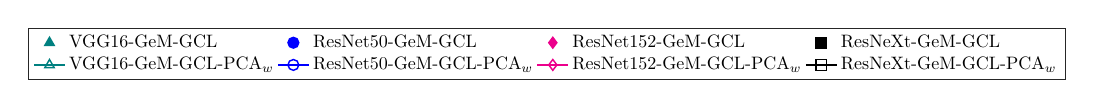
\begin{tikzpicture}[thick, scale=.65, every node/.style={scale=1}] 
    \begin{axis}[%
    hide axis,
    xmin=20,
    xmax=50,
    ymin=0,
    ymax=0.4,
    legend style={draw=white!15!black,legend cell align=left,legend columns=4}, height=4.75cm, width=.61\textwidth
    ]
\addlegendimage{teal,thick, mark=triangle*, mark size=3pt, only marks}
\addlegendentry{VGG16-GeM-GCL};
\addlegendimage{blue,thick, mark=*, mark size=3pt, only marks}
\addlegendentry{ResNet50-GeM-GCL};
\addlegendimage{magenta,thick, mark=diamond*, mark size=3pt, only marks}
\addlegendentry{ResNet152-GeM-GCL};
\addlegendimage{black,thick, mark=square*, mark size=3pt, only marks}
\addlegendentry{ResNeXt-GeM-GCL};

\addlegendimage{teal,thick, mark=triangle, mark size=3pt}
\addlegendentry{VGG16-GeM-GCL-PCA$_w$};

\addlegendimage{blue,thick, mark=o, mark size=3pt}
\addlegendentry{ResNet50-GeM-GCL-PCA$_w$};
\addlegendimage{magenta,thick, mark=diamond, mark size=3pt}
\addlegendentry{ResNet152-GeM-GCL-PCA$_w$};
\addlegendimage{black,thick, mark=square, mark size=3pt}
\addlegendentry{ResNeXt-GeM-GCL-PCA$_w$};

    \end{axis}
    \end{tikzpicture} 
  %  
\end{subfigure}
\end{minipage}

\begin{minipage}[c]{\textwidth}
\vspace{-30pt}
\setcounter{subfigure}{0}

\scriptsize
\begin{subfigure}{0.24\textwidth}
    %\subfloat[MSLS validation set]{
\begin{tikzpicture}[thick]
\begin{axis}
[xlabel=Dimensions,
ylabel=Recall@5 (\%), ylabel style={at={(axis description cs:0.2,0.5)}},grid, xmode=log,log basis x={2}, xtick={32,64,128,256, 512,1024,2048}, xticklabels={32,64,128,256, 512,1024,2048}, width=1.30\textwidth
]
\addplot[teal,thick, mark=triangle*, mark size=2pt] table [x=d, y=r, col sep=comma] {plot_data/whitening/MSLS/MSLS_soft_vgg16_GeM_L2_0-1_2_nowhiten_toplot};
\addplot[teal, mark=triangle, thick, mark size=2pt] table [x=d, y=r, col sep=comma] {plot_data/whitening/MSLS/MSLS_soft_vgg16_GeM_L2_0-1_2_whiten_toplot};
\addplot[blue,thick, mark=*, mark size=2pt] table [x=d, y=r, col sep=comma] {plot_data/whitening/MSLS/MSLS_soft_ResNet50_GeM_L2_0-1_2_nowhiten_toplot};
\addplot[blue, mark=o, thick, mark size=2pt] table [x=d, y=r, col sep=comma] {plot_data/whitening/MSLS/MSLS_soft_ResNet50_GeM_L2_0-1_2_whiten_toplot};
\addplot[magenta,thick, mark=diamond*, mark size=2pt] table [x=d, y=r, col sep=comma] {plot_data/whitening/MSLS/MSLS_soft_ResNet152_GeM_L2_0-1_2_nowhiten_toplot};
\addplot[magenta, mark=diamond, thick, mark size=2pt] table [x=d, y=r, col sep=comma] {plot_data/whitening/MSLS/MSLS_soft_ResNet152_GeM_L2_0-1_2_whiten_toplot};
\addplot[black,thick, mark=square*, mark size=2pt] table [x=d, y=r, col sep=comma] {plot_data/whitening/MSLS/MSLS_soft_resnext_GeM_L2_0-1_2_nowhiten_toplot};
\addplot[black, mark=square, thick, mark size=2pt] table [x=d, y=r, col sep=comma] {plot_data/whitening/MSLS/MSLS_soft_resnext_GeM_L2_0-1_2_whiten_toplot};
\end{axis}
 \label{fig:whitening_msls_val}
\end{tikzpicture}
\captionof{figure}{MSLS val}
\end{subfigure} \hspace{1.5mm}
%
\begin{subfigure}{0.24\textwidth}
    %\subfloat[MSLS test set]{
\begin{tikzpicture}[thick]
\begin{axis}
[xlabel=Dimensions, ,grid, xmode=log,log basis x={2}, xtick={32,64,128,256, 512,1024,2048}, xticklabels={32,64,128,256, 512,1024,2048}, width=1.30\textwidth
]
\addplot[teal,thick, mark=triangle*, mark size=2pt] table [x=d, y=r, col sep=comma] {plot_data/whitening/MSLS_test/MSLS_soft_vgg16_GeM_L2_0-1_2_nowhiten_toplot.txt};
\addplot[teal, mark=triangle, thick, mark size=2pt] table [x=d, y=r, col sep=comma] {plot_data/whitening/MSLS_test/MSLS_soft_vgg16_GeM_L2_0-1_2_whiten_toplot.txt};
\addplot[blue,thick, mark=*, mark size=2pt] table [x=d, y=r, col sep=comma] {plot_data/whitening/MSLS_test/MSLS_soft_ResNet50_GeM_L2_0-1_2_nowhiten_toplot.txt};
\addplot[blue, mark=o, thick, mark size=2pt] table [x=d, y=r, col sep=comma] {plot_data/whitening/MSLS_test/MSLS_soft_ResNet50_GeM_L2_0-1_2_whiten_toplot.txt};
\addplot[magenta,thick, mark=diamond*, mark size=2pt] table [x=d, y=r, col sep=comma] {plot_data/whitening/MSLS_test/MSLS_soft_ResNet152_GeM_L2_0-1_2_nowhiten_toplot.txt};
\addplot[magenta, mark=diamond, thick, mark size=2pt] table [x=d, y=r, col sep=comma] {plot_data/whitening/MSLS_test/MSLS_soft_ResNet152_GeM_L2_0-1_2_whiten_toplot.txt};
\addplot[black,thick, mark=square*, mark size=2pt] table [x=d, y=r, col sep=comma] {plot_data/whitening/MSLS_test/MSLS_soft_resnext_GeM_L2_0-1_2_nowhiten_toplot.txt};
\addplot[black, mark=square, thick, mark size=2pt] table [x=d, y=r, col sep=comma] {plot_data/whitening/MSLS_test/MSLS_soft_resnext_GeM_L2_0-1_2_whiten_toplot.txt};
\end{axis}
 \label{fig:whitening_msls_test}
\end{tikzpicture}
\captionof{figure}{MSLS test}
\end{subfigure} \hspace{0.5mm}
%
\begin{subfigure}{0.24\textwidth}
%\subfloat[Pitts30k test set]{
\begin{tikzpicture}[thick]
\begin{axis}
[xlabel=Dimensions,,grid, xmode=log,log basis x={2}, xtick={32,64,128,256, 512,1024,2048}, xticklabels={32,64,128,256, 512,1024,2048}, width=1.30\textwidth
]
\addplot[teal,thick, mark=triangle*, mark size=2pt] table [x=d, y=r, col sep=comma] {plot_data/whitening/Pitts30k/MSLS_soft_vgg16_GeM_L2_0-1_2_nowhiten_toplot};
\addplot[teal, mark=triangle, thick, mark size=2pt] table [x=d, y=r, col sep=comma] {plot_data/whitening/Pitts30k/MSLS_soft_vgg16_GeM_L2_0-1_2_whiten_toplot};
\addplot[blue,thick, mark=*, mark size=2pt] table [x=d, y=r, col sep=comma] {plot_data/whitening/Pitts30k/MSLS_soft_ResNet50_GeM_L2_0-1_2_nowhiten_toplot};
\addplot[blue, mark=o, thick, mark size=2pt] table [x=d, y=r, col sep=comma] {plot_data/whitening/Pitts30k/MSLS_soft_ResNet50_GeM_L2_0-1_2_whiten_toplot};
\addplot[magenta,thick, mark=diamond*, mark size=2pt] table [x=d, y=r, col sep=comma] {plot_data/whitening/Pitts30k/MSLS_soft_ResNet152_GeM_L2_0-1_2_nowhiten_toplot};
\addplot[magenta, mark=diamond, thick, mark size=2pt] table [x=d, y=r, col sep=comma] {plot_data/whitening/Pitts30k/MSLS_soft_ResNet152_GeM_L2_0-1_2_whiten_toplot};
\addplot[black,thick, mark=square*, mark size=2pt] table [x=d, y=r, col sep=comma] {plot_data/whitening/Pitts30k/MSLS_soft_resnext_GeM_L2_0-1_2_nowhiten_toplot};
\addplot[black, mark=square, thick, mark size=2pt] table [x=d, y=r, col sep=comma] {plot_data/whitening/Pitts30k/MSLS_soft_resnext_GeM_L2_0-1_2_whiten_toplot};
\end{axis}
 \label{fig:whitening_pitts30k}
\end{tikzpicture}
\captionof{figure}{Pitts30k}
\end{subfigure} \hspace{0.5mm}
%
\begin{subfigure}{0.24\textwidth}
%\subfloat[Tokyo 24/7]{
\begin{tikzpicture}[thick]
\begin{axis}
[xlabel=Dimensions, ylabel style={at={(axis description cs:-0.08,0.5)}},grid, xmode=log,log basis x={2}, xtick={32,64,128,256, 512,1024,2048}, xticklabels={32,64,128,256, 512,1024,2048}, width=1.30\textwidth
]
\addplot[teal,thick, mark=triangle*, mark size=2pt] table [x=d, y=r, col sep=comma] {plot_data/whitening/Tokyo247/MSLS_soft_vgg16_GeM_L2_0-1_2_nowhiten_toplot};
\addplot[teal, mark=triangle, thick, mark size=2pt] table [x=d, y=r, col sep=comma] {plot_data/whitening/Tokyo247/MSLS_soft_vgg16_GeM_L2_0-1_2_whiten_toplot};
\addplot[blue,thick, mark=*, mark size=2pt] table [x=d, y=r, col sep=comma] {plot_data/whitening/Tokyo247/MSLS_soft_ResNet50_GeM_L2_0-1_2_nowhiten_toplot};
\addplot[blue, mark=o, thick, mark size=2pt] table [x=d, y=r, col sep=comma] {plot_data/whitening/Tokyo247/MSLS_soft_ResNet50_GeM_L2_0-1_2_whiten_toplot};
\addplot[magenta,thick, mark=diamond*, mark size=2pt] table [x=d, y=r, col sep=comma] {plot_data/whitening/Tokyo247/MSLS_soft_ResNet152_GeM_L2_0-1_2_nowhiten_toplot};
\addplot[black,thick, mark=square*, mark size=2pt] table [x=d, y=r, col sep=comma] {plot_data/whitening/Tokyo247/MSLS_soft_resnext_GeM_L2_0-1_2_nowhiten_toplot};

\addplot[magenta, mark=diamond, thick, mark size=2pt] table [x=d, y=r, col sep=comma] {plot_data/whitening/Tokyo247/MSLS_soft_ResNet152_GeM_L2_0-1_2_whiten_toplot};

\addplot[black, mark=square, thick, mark size=2pt] table [x=d, y=r, col sep=comma] {plot_data/whitening/Tokyo247/MSLS_soft_resnext_GeM_L2_0-1_2_whiten_toplot};
\end{axis}
\label{fig:whitening_tokyo247}
\end{tikzpicture}
\captionof{figure}{Tokyo24/7}
\end{subfigure}
\end{minipage}

\vspace{-2mm}    \caption{Ablation results on the MSLS validation, MSLS test, Pittsburgh30k and Tokyo 24/7 datasets, with different PCA dimensions.}
    \label{fig:whitening}
\end{figure*}






\noindent\textbf{Generalization to other datasets. } In Table~\ref{tab:msls-sota} and Table~\ref{tab:msls-ablation}, we also report the results of generalization to Pittsburgh30k, Tokyo 24/7, RobotCar Seasons v2 and Extended CMU Seasons (plus Pittsburgh250k and TokyoTM in the supplementary materials). The models trained with the GCL function generalize well to unseen datasets, in many cases better than existing methods that retrieve the $k$-nearest neighbours based on  descriptor distance only. %, despite using descriptors of lower dimensionality. 
%
%In the case of Pittsburgh30k, our models achieve competitive results, up to 91.5\% top-5 recall, which is very close to the 91.8\% reported by NetVLAD-64 trained on the Pittsburgh30k dataset itself, and slightly lower than re-ranking methods such as TransVPR (top-5 recall of 94.9\%) and Patch-NetVLAD (top-5 recall of 94.5\%). 
%
%
Our models also generalize well to urban localization datasets like RobotCar Seasons V2 and Extended CMU Seasons, achieving up to 21.9\% and 19\% of correctly localized queries within 0.5m and 5$\degree$, respectively. The results of GCL-based networks are higher than those obtained by NetVLAD, and especially higher than those of TransVPR (with no re-ranking) that uses a transformer as backbone. Note that we do not perform 6DOF pose estimation, but estimate the pose of a query image by inheriting that of the best retrieved match, and thus not compare with methods that perform refined pose estimation. This is inline with the experiments in~\cite{hausler2021patch}. %, while being lower than those of NetVLAD trained on Pittsburgh and 

Our models are outperformed only by methods that include a re-ranking strategies to refine the list of retrieved images, on the Pittsburgh30k, RobotCar Seasons v2 and Extended CMU Seasons datasets. However, these methods perform extra heavy computations (e.g. up to $6s$ per query in PatchNetVLAD~\cite{hausler2021patch}) to re-rank the list of retrieved images, not focusing on the representation capabilities of the learned descriptors themselves. Thus, we find a direct comparison with these methods not fair. On the contrary, these results demonstrate the fact the VPR descriptors learned used the proposed labels and GCL have better representation capabilities than those produced by other methods, achieving higher results in out-of-distribution experiments as well.

%the re-ranking based Patch-NetVLAD. , while achieving superior performance w.r.t. methods that, similarly to ours, retrieve the $k$-nearest neighbours only based on the descriptor distance. This indicates that the GCL metric learning contributes to latent representations that are robust to domain shifts and can generalize well to other datasets and environments.






\noindent\textbf{Ablation study: backbone and contrastive loss. } We carried out ablation experiments using four backbones, namely VGG16~\cite{simonyan2015very}, ResNet50, ResNet152~\cite{he2016deep}, and ResNeXt101-32x8d (hereinafter ResNeXt)~\cite{xie2017aggregated}, and the GeM~\cite{radenovic2018fine} global pooling layer, and an additional NetVLAD-GCL model. Extra ablation experiments with an average global pooling layer are included in the supplementary material. For each backbone, we train with the binary Contrastive Loss (CL) and our Generalized Contrastive Loss (GCL). We report the results in Table~\ref{tab:msls-ablation}. The models trained with the GCL consistently outperform their counterpart trained with the CL, showing better generalization to other datasets. Moreover, we demonstrate that a VGG16-GeM architecture outperforms a more complex NetVLAD when trained with our GCL function.  We also perform whitening and PCA on the descriptors, which further boost the performance.
% we report the results of the ablation studyand Fig.~\ref{fig:msls_recall}, the models trained with the GCL function consistently outperform their counterparts trained with the CL. 

%For \revised{all models}, we also perform a postprocessing step consisting of PCA whitening and observe that it further boosts the performance. 
\noindent\textbf{Ablation study: PCA and whitening. } We also study the effect of whitening and PCA dimensionality reduction from 32 to 2048 dimensions. Figure~\ref{fig:whitening} shows the results on the MSLS, Pittsburgh30k and Tokyo 24/7 datasets. In general, the larger the size of the descriptors, the better the results. However, our models maintain comparably high results when the descriptors are whitened and reduced to 256 dimensions, still outperforming the full-size descriptors without whitening. We observed up to a $28.2\%$ improvement in the case of Tokyo 24/7 and $12.8\%$ on the MSLS validation set. When comparing our VGG16-GeM-GCL model reduced to 256 dimensions with NetVLAD ($16\times$ less descriptor size), we still achieve higher results (R@5 of 82.7\% vs 80.8\% on MSLS validation, 60.4\% vs 58.9\% on MSLS test, 87.2\% vs 84.7\% on Pittsburg30k and 62.2\% vs 47.6\% on Tokyo 24/7).
It is to highlight that the contributions of the PCA/whitening and the GCL are complementary, meaning that they can be used together to optimize retrieval performance.
%The whitened descriptors with higher dimensionality achieve \revised{better} results.

%It is worth noting that the ResNeXt-GeM-GCL maintains the same performance when reduced down to 256 dimensions, and that VGG16-GeM-GCL reaches peak top-5 recall when reduced to 256 features. 
%When using the whitening transform combined with PCA dimensionality reduction down to 128 dimensions of the latent space, our models achieved results comparable to those of \revised{models with full-size dimensions (2048 for ResNet and ResNeXt, and 512 for VGG)}, which outperform their non-whithened counterpart on all the considered datasets. We observed up to a 28.2\% of improvement in the case of Tokyo 24/7 and 12.8\% on the MSLS validation set.
%\ns{comment on effect of GCL and effect of PCA, which are complementary.}

\newcommand{\dashrule}[1][black]{%
  \color{#1}\rule[\dimexpr.5ex-.2pt]{4pt}{.4pt}\xleaders\hbox{\rule{4pt}{0pt}\rule[\dimexpr.5ex-.2pt]{4pt}{.4pt}}\hfill\kern0pt%
}

\begin{table*}[!t]
\renewcommand{\arraystretch}{1.05}
\setlength\tabcolsep{1.5pt}
\centering
\caption{Comparison of localization results (on CMU Seasons) of VGG16 backbones trained with several metric loss functions. Methods in the upper part deploy a NetVLAD pooling layer.}
\label{tab:comparisonwiththoma}
\resizebox{\textwidth}{!}{%
\footnotesize

\begin{tabular} {l@{\hspace{16\tabcolsep}}ccc@{\hspace{20\tabcolsep}}ccc@{\hspace{14\tabcolsep}}ccc@{\hspace{14\tabcolsep}}ccc}
\toprule
 & \multicolumn{3}{c}{\textbf{All}} & \multicolumn{3}{c}{\textbf{Urban}} & \multicolumn{3}{c}{\textbf{Suburban}} & \multicolumn{3}{c}{\textbf{Park}} \\ 
\textbf{Loss function} & \textbf{0.25m/2$\degree$} & \textbf{0.5m/5$\degree$} & \textbf{5m/10$\degree$} & \textbf{0.25m/2$\degree$} & \textbf{0.5m/5$\degree$} & \textbf{5m/10$\degree$} & \textbf{0.25m/2$\degree$} & \textbf{0.5m/5$\degree$} & \textbf{5m/10$\degree$} & \textbf{0.25m/2$\degree$} & \textbf{0.5m/5$\degree$} & \textbf{5m/10$\degree$} \\\midrule
%Off-the-shelf~\cite{Arandjelovic2017} & 4.7 & 11.8 & 42.0 & 7.8 & 18.5 & 54.9 & 2.9 & 8.5 & 36.2 & 2.6 & 6.8 & 32.0  \\
%Triplet trained on Pittsburgh~\cite{Arandjelovic2017} & 5.3 & 13.3 & 48.2  & 9.1 & 21.5 & 64.3 & 3.2 & 9.5 & 45.0 & 2.5 & 6.9 & 32.7  \\
Triplet (original NetVLAD)~\cite{Arandjelovic2017} & 6.0 & 15.5 & 59.9  &  9.4 & 22.6 & 71.2 & 3.9 & 11.8 & 60.1 & 3.2 & 9.2 & 45.2    \\
Quadruplet~\cite{Chen2017beyondTriplet} & 6.9 & 17.5 & 62.3  & 10.7 & 25.2 & 73.3 & 4.4 & 13.0 & 61.4 & 3.9 & 10.8 & 47.9    \\
Lazy triplet~\cite{angelina2018pointnetvlad} & 6.4 & 16.5 & 58.6  &  9.9 & 23.5 & 69.8 & 4.1 & 11.9 & 58.2 & 3.5 & 10.1 & 42.0  \\
Lazy quadruplet~\cite{angelina2018pointnetvlad} & 7.3 & 18.5 & 61.7  & 11.4 & 26.9 & 72.7 & 4.9 & 13.9 & 64.1 & 3.7 & 10.7 & 44.1  \\
Triplet + Huber distance~\cite{Thoma2020Mappable} & 6.0 & 15.3 & 55.9 & 9.5 & 22.9 & 69.0 & 4.4 & 12.4 & 57.3 & 3.0 & 8.4 & 39.6   \\
Log-ratio~\cite{kim2019deep} & 6.7 & 17.4 & 58.8  & 10.5 & 24.9 & 71.4 & 4.6 & 13.4 & 57.4 & 3.5 & 10.2 & 42.8  \\
Multi-similarity~\cite{Wang2019multisimilarity} & 7.4 & 18.8 & 66.3 & 12.0 & 28.8 & 81.6 & 5.1 & 14.6 & 63.9 & 3.8 & 10.9 & 52.7 \\
Soft contrastive~\cite{thoma2020soft} & 8.0 & 20.5 & \bfseries 70.4 & 12.7 & 30.7 & \bfseries 84.6 & 5.1 & 14.9 & \bfseries 67.9 & 4.5 & 12.6 & \bfseries 56.8 \\ \midrule
%VGG-GeM-GCL & 5.9 & 15.4 & 58.9 & 9.6 & 24.1 & 76.4 & 3.1 & 9.8 & 56.3 & 3.3 & 9.0 & 42.0 \\
\bfseries GCL (Ours) & \bfseries 9.2 & \bfseries 22.8 & 65.8 & \bfseries 14.7 & \bfseries 34.2 & 82.6 & \bfseries 5.7 & \bfseries 16.1 & 64.6 & \bfseries 5.1 & \bfseries 14.0 & 49.1 \\ \tabucline[0.4pt black!40 off 2pt]{~}
\textit{GCL (Ours w/ ResNeXt)} & \textit{9.9} & \textit{24.3} & \textit{75.5} & \textit{15.4} & \textit{36.0} & \textit{89.6} & \textit{6.7} & \textit{18.4} & \textit{76.8} & \textit{5.6} & \textit{14.9} & \textit{60.3} \\ 
\bottomrule
\end{tabular}%
}
\end{table*}

%Resnet50-GeM-GCL & 6.3 & 16.3 & 62.8 & 10.4 & 25.5 & 81.2 & 3.8 & 11.2 & 63.9 & 3.2 & 9.0 & 43.3 \\
%Resnet50-GeM-GCL+PCA$_w$ & 9.0 & 22.5 & 69.3 & 14.3 & 33.8 & 85.1 & 6.1 & 17.0 & 71.1 & 4.9 & 13.4 & 52.2 \\
%Resnet152-GeM-GCL & 6.2 & 16.2 & 66.2 & 10.1 & 24.8 & 82.0 & 4.1 & 12.2 & 66.4 & 3.1 & 9.2 & 49.9 \\
%Resnet152-GeM-GCL+PCA$_w$ & 8.8 & 21.6 & 64.0 & 14.1 & 32.4 & 80.0 & 5.9 & 16.8 & 65.2 & 4.7 & 12.7 & 47.0 \\
%GCL (Ours) & 5.8 & 15.1 & 63.0 & 9.5 & 24.0 & 81.0 & 3.5 & 10.5 & 62.5 & 2.9 & 7.9 & 44.7 \\







\noindent\textbf{Comparison with other loss functions. } We compared with other loss functions used for VPR, by following up on the experiments in~\cite{thoma2020soft}. % , we use the CMU Season dataset~\cite{Badino2011}. 
The loss functions included in the comparison in~\cite{thoma2020soft} are the triplet loss~\cite{Arandjelovic2017} (also with Huber distance~\cite{Thoma2020Mappable}), quadruplet loss~\cite{Chen2017beyondTriplet}, lazy triplet and lazy quadruplet loss~\cite{angelina2018pointnetvlad}, plus functions that embed mechanisms to circumvent the use of binary labels, namely a multi-similarity loss~\cite{Wang2019multisimilarity}, log-ratio~\cite{kim2019deep} and soft contrastive loss~\cite{thoma2020soft}. 
The results reported in Table~\ref{tab:comparisonwiththoma} show that the GCL achieves higher localization accuracy especially when stricter thresholds for distance and angle are set. These results indicate that the GCL descriptors are better effective in neighbor search and retrieval, and their ranking based on distance from the query descriptor is a more reliable measure of visual place similarity. %They are trained so that their distance is a .
All methods in the upper part of the table deploy a VGG16 backbone with a NetVLAD pooling layer and make use of hard-negative pair mining. We also use a VGG16 backbone and do not perform hard-negative pair mining, substantially reducing the training time and memory requirements. This allows us to also train backbones with larger capacity, e.g. ResNeXt, on a single V100 GPU in less than a day, of which we report the results in italics for completeness.






\noindent\textbf{Processing time. } The GCL function and the graded similarity labels contribute to training effective models in a data- and computation-efficient way, largely improving on the resources and time required to train NetVLAD (see Table~\ref{tab:training-time}). Our VGG16-GeM-GCL model obtains higher results than NetVLAD while requiring $6\times$ less memory and about $100\times$ less time to converge. We point out that NetVLAD is the backbone of several other methods for VPR such as PatchNetVLAD, DELG and SuperGlue in Table~\ref{tab:msls-sota}, thus making the comparison in Table~\ref{tab:training-time} relevant from a larger perspective.
The graded similarity and GCL function contribute to an efficient use of training data. A single epoch, i.e. a model sees a certain training pair only once, is sufficient for the training of GCL-based models to converge. The low memory and time requirements also enable the training of models with larger backbones, that obtain very high results while still keeping the resource usage low.
We point out the data-efficient training that we deployed can stimulate further and faster progress in VPR, as it enables to train larger backbones, and perform extensive hyperparameter optimization or more detailed ablation studies.

%more efficient way than NetVLAD-based ones, as shown in Table~\ref{tab:training-time}. The training time per epoch of our models is less than that of NetVLAD, as we do not perform hard-pair mining. Furthermore, we train our GCL models for only one epoch on the MSLS dataset, while NetVLAD-16 and NetVLAD-64 converged after 22 and 7 epochs, respectively.



\begin{table}[t!]
\centering
\revised{\caption{Training time and GPU memory utilization for a batch size of 4 images. In the epochs column, the number in parenthesis is the number of epochs until convergence. }
\label{tab:training-time}
\footnotesize
%\resizebox{\columnwidth}{!}{%
\begin{tabular}{@{}lcccc@{}}
\toprule
\textbf{Model} &\textbf{memory} & \textbf{epochs} & \textbf{t/epoch} & \textbf{t/converge} \\ \midrule
NetVLAD-16-TL & 9.67GB & 30 (22) & 24h & 22d \\
NetVLAD-64-TL & - &10 (7) & 36h & 10.5d \\
VGG16-GeM-GCL & 1.49GB & 1 & 5h & 5h \\
ResNet50-GeM-GCL & 1.65 GB & 1 & 6h & 6h \\
ResNet152-GeM-GCL & 3.78 GB & 1 & 14h & 14h \\
ResNetXt-GeM-GCL & 4.77 GB& 1 (1/2) & 28h & 14h \\ \bottomrule
\end{tabular}%
}%}
\end{table}







%\noindent\textbf{Partial training of backbones. }


%\noindent\textbf{Limitations.}\label{sec:limitations} We have demonstrated that the GCL function allows the training of contrastive architectures effectively and efficiently, obtaining higher results than SoA triplet networks. The results are attributable to the exploitation of the graded similarity of the input pairs to train the networks. However, the availability of suitable extra data to compute a graded similarity is a limitation for the training using the GCL function. For instance, the images in the Pittsburgh30k dataset are provided with the GPS coordinates only, with no camera orientation information. This prevents from computing the FoV of the cameras and their overlap, thus limiting the use of the GCL function to train on Pittsburgh30k and similar datasets. 

